\documentclass{article}
\usepackage[margin=1in]{geometry}
\usepackage{graphicx}
\usepackage{caption}
\usepackage{subcaption}
\usepackage{float}
\usepackage{amsmath}
\usepackage{booktabs}

\setcounter{secnumdepth}{0}

\title{Memory masking vs overwriting in procedural categorization}
\author{}
\date{}

\begin{document}

\maketitle

\section{Intro}
In an era defined by ubiquitous digital devices and a
seemingly endless stream of media optimized to hijack our
attention, the ability to manage, redirect, or erase
habitual behavior is more critical than ever. Technological
advances have dramatically enhanced the capacity of product
developers to induce habitual use, yet our ability to
flexibly control or disrupt these behaviors has failed to
keep pace. This growing imbalance poses serious
challenges—not only to individual well-being but also to the
functioning of society—and addressing it is increasingly
important.

A major source of habitual behavior likely lies in the
neural mechanisms supporting operant stimulus-response (SR)
learning. In the animal learning literature, especially in
rodent models, behavior is often characterized along a
continuum from goal-directed to habitual. Goal-directed
actions are sensitive to the agent’s current goals and
motivational states, enabling flexible adaptation to
changing environmental contingencies. In contrast, habitual
behaviors are rigid and automatic—triggered directly by
environmental cues—and often persist even when the
associated reward is devalued. For example, a rat may
continue pressing a lever for food despite being sated, much
like a human may continue scrolling through social media
absent any specific goal or gratification.

In the human cognitive literature, this distinction between
goal-directed and habitual behavior closely parallels the
division between declarative and procedural learning and
memory systems. Declarative memory supports flexible,
hypothesis-driven reasoning and explicit knowledge, while
procedural memory underlies behaviors learned through direct
reinforcement and repeated experience, typically with little
cognitive effort or conscious awareness. This division is
particularly well studied in the domain of category
learning, where different category structures are thought to
preferentially engage different memory systems.

In recent work, we reported an intervention that appeared to
induce true overwriting of procedural category knowledge.
Participants who had previously acquired a category
structure through procedural learning no longer showed
evidence of this knowledge following the intervention,
suggesting that the learned associations had been erased.
However, a critical alternative explanation remained
untested. Rather than eliminating the procedural memory, the
intervention may have merely masked its behavioral
expression. On this account, the underlying SR mappings
remain intact but lie dormant and may reemerge under
appropriate conditions.

In the present study, we directly test this possibility. We
provide clear evidence that the intervention does not result
in unlearning of procedural category knowledge. Instead, it
masks the expression of that knowledge, which remains
accessible under suitable retrieval conditions. These
findings have important implications for how we understand,
measure, and intervene on habit-like behaviors across
domains.

\section{Methods}

\subsection{Experiments and conditions}
The study consisted of two experiments, each comprising
three phases: Learn, Intervention, and Test. In both
experiments, participants were assigned to one of two
between-subject conditions: Relearn or New Learn. The Learn
and Test phases were identical across experiments and
conditions. During the Learn phase, participants were
trained on a category structure designed to promote
procedural learning. In the Test phase, they were assessed
on the same or a new category structure, depending on their
assigned condition. The critical manipulation occurred
during the Intervention phase. In Experiment~1, participants
received fully random feedback during this phase, whereas in
Experiment~2, feedback was a mixture of random and
veridical. This design allowed us to assess whether the
interventions disrupted or merely masked previously acquired
procedural knowledge.

\subsection{Stimuli and categories}
The stimuli were circular sine-wave gratings that varied in
spatial frequency and orientation.  The coordinates of all
stimuli were generated by first sampling points in polar
coordinates and then converting them into Cartesian
coordinates.  Specifically, radius values $r$ were sampled
from a uniform distribution on the interval $[0, 1]$, and
angle values $\theta$ were sampled uniformly from the
interval $[0, 2\pi]$.  These polar coordinates $(r, \theta)$
were then transformed into Cartesian coordinates $(x, y)$
using the equations $x = r \cos(\theta)$ and $y =
r\sin(\theta)$. This resulted in a set of $(x, y)$
coordinates uniformly distributed within a circle of radius
1 and centered at the origin. Next, $(x,y)$ coordinates were
transformed from a circular uniform distribution to an
elliptical uniform distribution with horizontal major axis
by multiplying the $x$ values by 124.02 and the $y$ values
by 28.44. For the Test phase in the New Learning conditions,
the resulting coordinates were rotated by 45\degree and
translated by $(40, 60)$ for half the stimuli and by $(60,
40)$ for the other half. The resulting stimulus
distributions are shown in Figure~\ref{fig_cat}.

\begin{figure}[H]
    \centering
    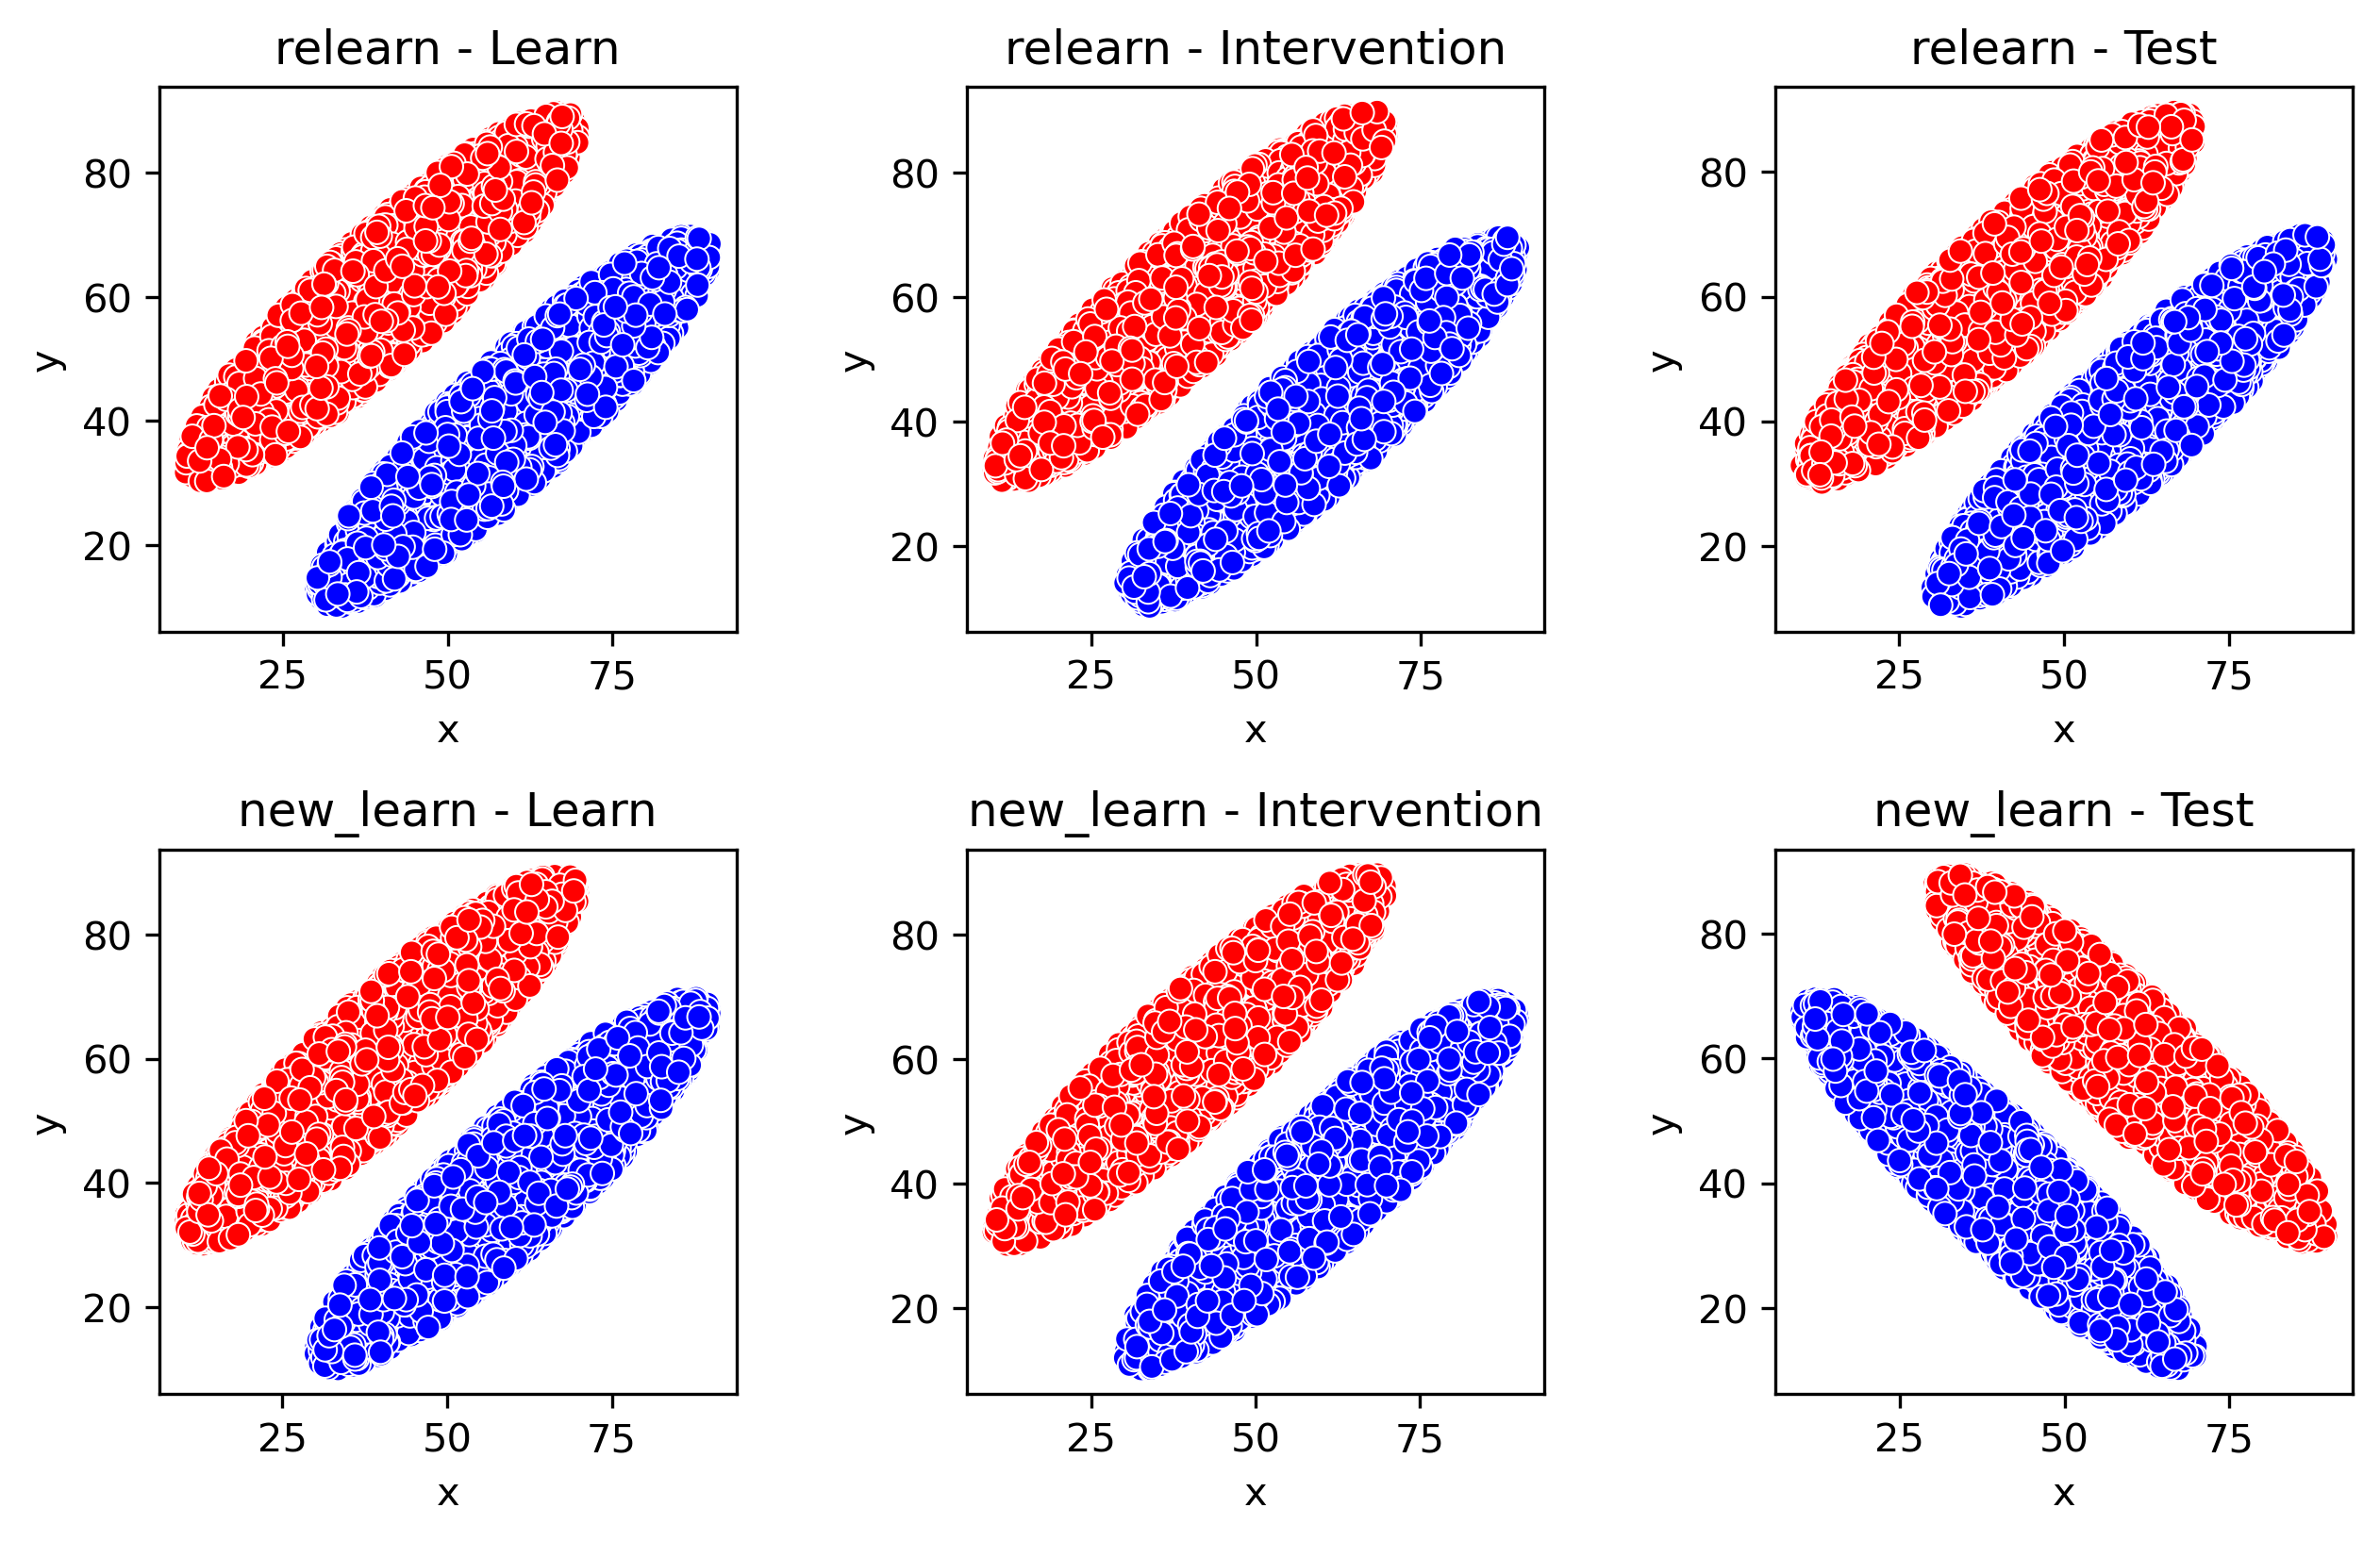
\includegraphics[width=\textwidth]{../figures/fig_cat_struct.png}
    \caption{}
    \label{fig_cat}
\end{figure}

Category learning can be described within a multiple-systems
framework that distinguishes between declarative and
procedural mechanisms \citep{ashby1998differentiating,
ashby2017multiple}.  Declarative category learning relies on
explicit reasoning and hypothesis testing. Rule-based (RB)
tasks are commonly used to study this system, as they
typically require participants to apply simple, verbally
describable rules (e.g., ``if orientation exceeds a
threshold, choose Category A; otherwise, Category B'';
\citealp{filoteo2005, nomura2007neural}).

Procedural category learning, by contrast, depends on the
gradual formation of stimulus--response associations
acquired through reinforcement of direct experience.
Information-integration (II) tasks are typically used to
study this system. These tasks require learners to combine
information across multiple stimulus dimensions in a way
that cannot be easily verbalized. Unlike RB learning, where
performance often improves suddenly following discovery of
the correct rule, II learning is characterized by
incremental trial-by-trial improvements
\citep{maddox2004dissociating, ashby2011}.

Evidence for the RB tasks are primarily learned with
declarative systems and II learning is primarily learned
with procedural systems comes from behavioral, neuroimaging,
and patient studies (for reviews, see REF). In the present
study, we employ II categories because they specifically
engage procedural mechanisms, thereby providing a window
into the stimulus--response processes that underlie broader
habitual behaviors.

\subsection{Procedure}
Participants provided informed consent and were given an
optional demographic questionnaire to complete. Participants
were instructed that their task was to categorize circular
sine-wave gratings on the basis of their spatial frequency
and orientation, and that each category was equally likely.

Each participant completed a single session consisting of
900 trials. Each phase (Learn, Intervention, Test) consisted
of 300 trials. On each trial, participants viewed a fixation
cross (1000 ms), followed by a response-terminated stimulus,
and then feedback (1000 ms).  Responses were given via the
``d'', and ``k'' keys.  Feedback following correct responses
was a green circle that appeared around the stimulus, and
feedback following incorrect responses was a red circle. See
Figure~\ref{fig_example_trials} an illustration of example
trials.

\subsection{Participants}
A total of 40 participants were recruited for Experiment 1
(32 female, 8 male), with ages ranging from 18 to 32 years
(M = 20.33, SD = 2.61). An additional 40 participants took
part in Experiment 2 (X female, X male, 2 nonbinary, and 1
preferred not to disclose), with ages ranging from X to X
years (M = X, SD = X). Participants were pseudo-randomly
assigned to either the new learning or relearning condition
using a blocked allocation method, ensuring equal sample
sizes (n = 20) in each condition. To be eligible,
participants had to be at least 18 years old with normal or
corrected-to-normal vision. All participants were
undergraduate students at Macquarie University and received
course credit in exchange for participation. Ethics approval
for this study was granted by the Macquarie University Human
Research Ethics Committee (Ref: 520251317762011).

\subsection{Decision-Bound Analysis}
To identify the decision strategy used by each participant,
we fit decision-bound models \parencite{AshbyValentin2018}
to the trial-by-trial response data from the final 100
trials of the Train phase and the first 100 trials of the
Test phase separately for each participant. We examined
1-dimensional rule-based models and 2-dimensional procedural
models.  The rule-based models assumed participants
established a criterion on a single stimulus dimension and
then categorized stimuli based on whether or not they
exceeded this criterion. These models had two free
parameters -- a response criterion on the attended stimulus
dimension, and the variance of perceptual and criterial
noise. The 2-dimensional procedural models -- i.e., general
linear classifier (GLC) --  assumed that participants used a
linear decision boundary with an arbitrary slope and
intercept to divide the stimulus space into two response
regions. The GLC assumes that stimuli are categorized based
on their position relative to this boundary. The GLC has
three free parameters -- a slope and intercept of the
decision bound and the variance of perceptual and criterial
noise. For details on the models and the model-fitting
process, see \textcite{AshbyValentin2018}.

\subsection{Bayesian Estimation of Procedural Reacquisition}
To estimate and compare the probability that participants
reacquired a procedural strategy across experiments and
conditions, we conducted a series of Bayesian analyses using
posterior sampling from Beta distributions. 

We defined reacquisition as participants being classified as
procedural in both the initial learning phase (Block 2) and
the final test phase (Block 6). For each condition (Relearn
vs.\ New Learning) and experiment (Experiment 1 vs.\
Experiment 2), we computed the posterior distribution over
the reacquisition probability, $\theta$, using a Beta prior
with parameters $\alpha = 1$ and $\beta = 1$ (i.e., a
uniform prior). Given the observed number of procedural
reacquisitions (successes) and total participants in each
group, we drew 100{,}000 samples from the resulting Beta
posterior distribution for each group:

\begin{equation}
\theta \sim \mathrm{Beta}(\text{successes} + 1,\ \text{failures} + 1)
\end{equation}

For each condition, we then computed the posterior
distribution over the difference in reacquisition
probability between Experiment 1 and Experiment 2 by
subtracting posterior samples ($\Delta = \theta_1 -
\theta_2$). We derived 95\% credible intervals from these
difference distributions and reported the posterior
probability that $\Delta > 0$ (i.e., the probability that
reacquisition was more likely in Experiment 1 than in
Experiment 2).

Additionally, to assess the effect of condition within each
experiment, we compared the posterior distributions of
reacquisition rates between the Relearn and New Learning
conditions separately for Experiment 1 and Experiment 2.

The resulting posterior distributions and their differences
were visualized using histograms, with red dashed lines
indicating 95\% credible intervals and black dashed lines
marking the null value ($\Delta = 0$). This analysis
provides direct probabilistic evidence about the likelihood
of differences in reacquisition rates across experiments and
conditions.

\section{Results}
Figure~\ref{fig_learning_curves} displays mean accuracy per
block for each condition and experiment. In Experiment 1
(left panel), participants successfully learned the category
structure during the Learn phase but ceased to express this
knowledge during the Intervention phase. During the Test
phase, participants in the Relearn condition rapidly
returned to their previous accuracy levels, indicating that
the intervention (random feedback) did not erase the
original learning. In contrast, those in the New Learn
condition performed significantly worse, consistent with
interference from the previously learned, conflicting
stimulus-response mappings. A similar pattern was observed
in Experiment 2 (right panel), suggesting that a
mixed-feedback intervention failed to overwrite the initial
learning. These findings support the interpretation that the
mixed feedback intervention results we previously reported
on masked, rather than erased, procedural category
knowledge.

\begin{figure}[H]
    \centering
    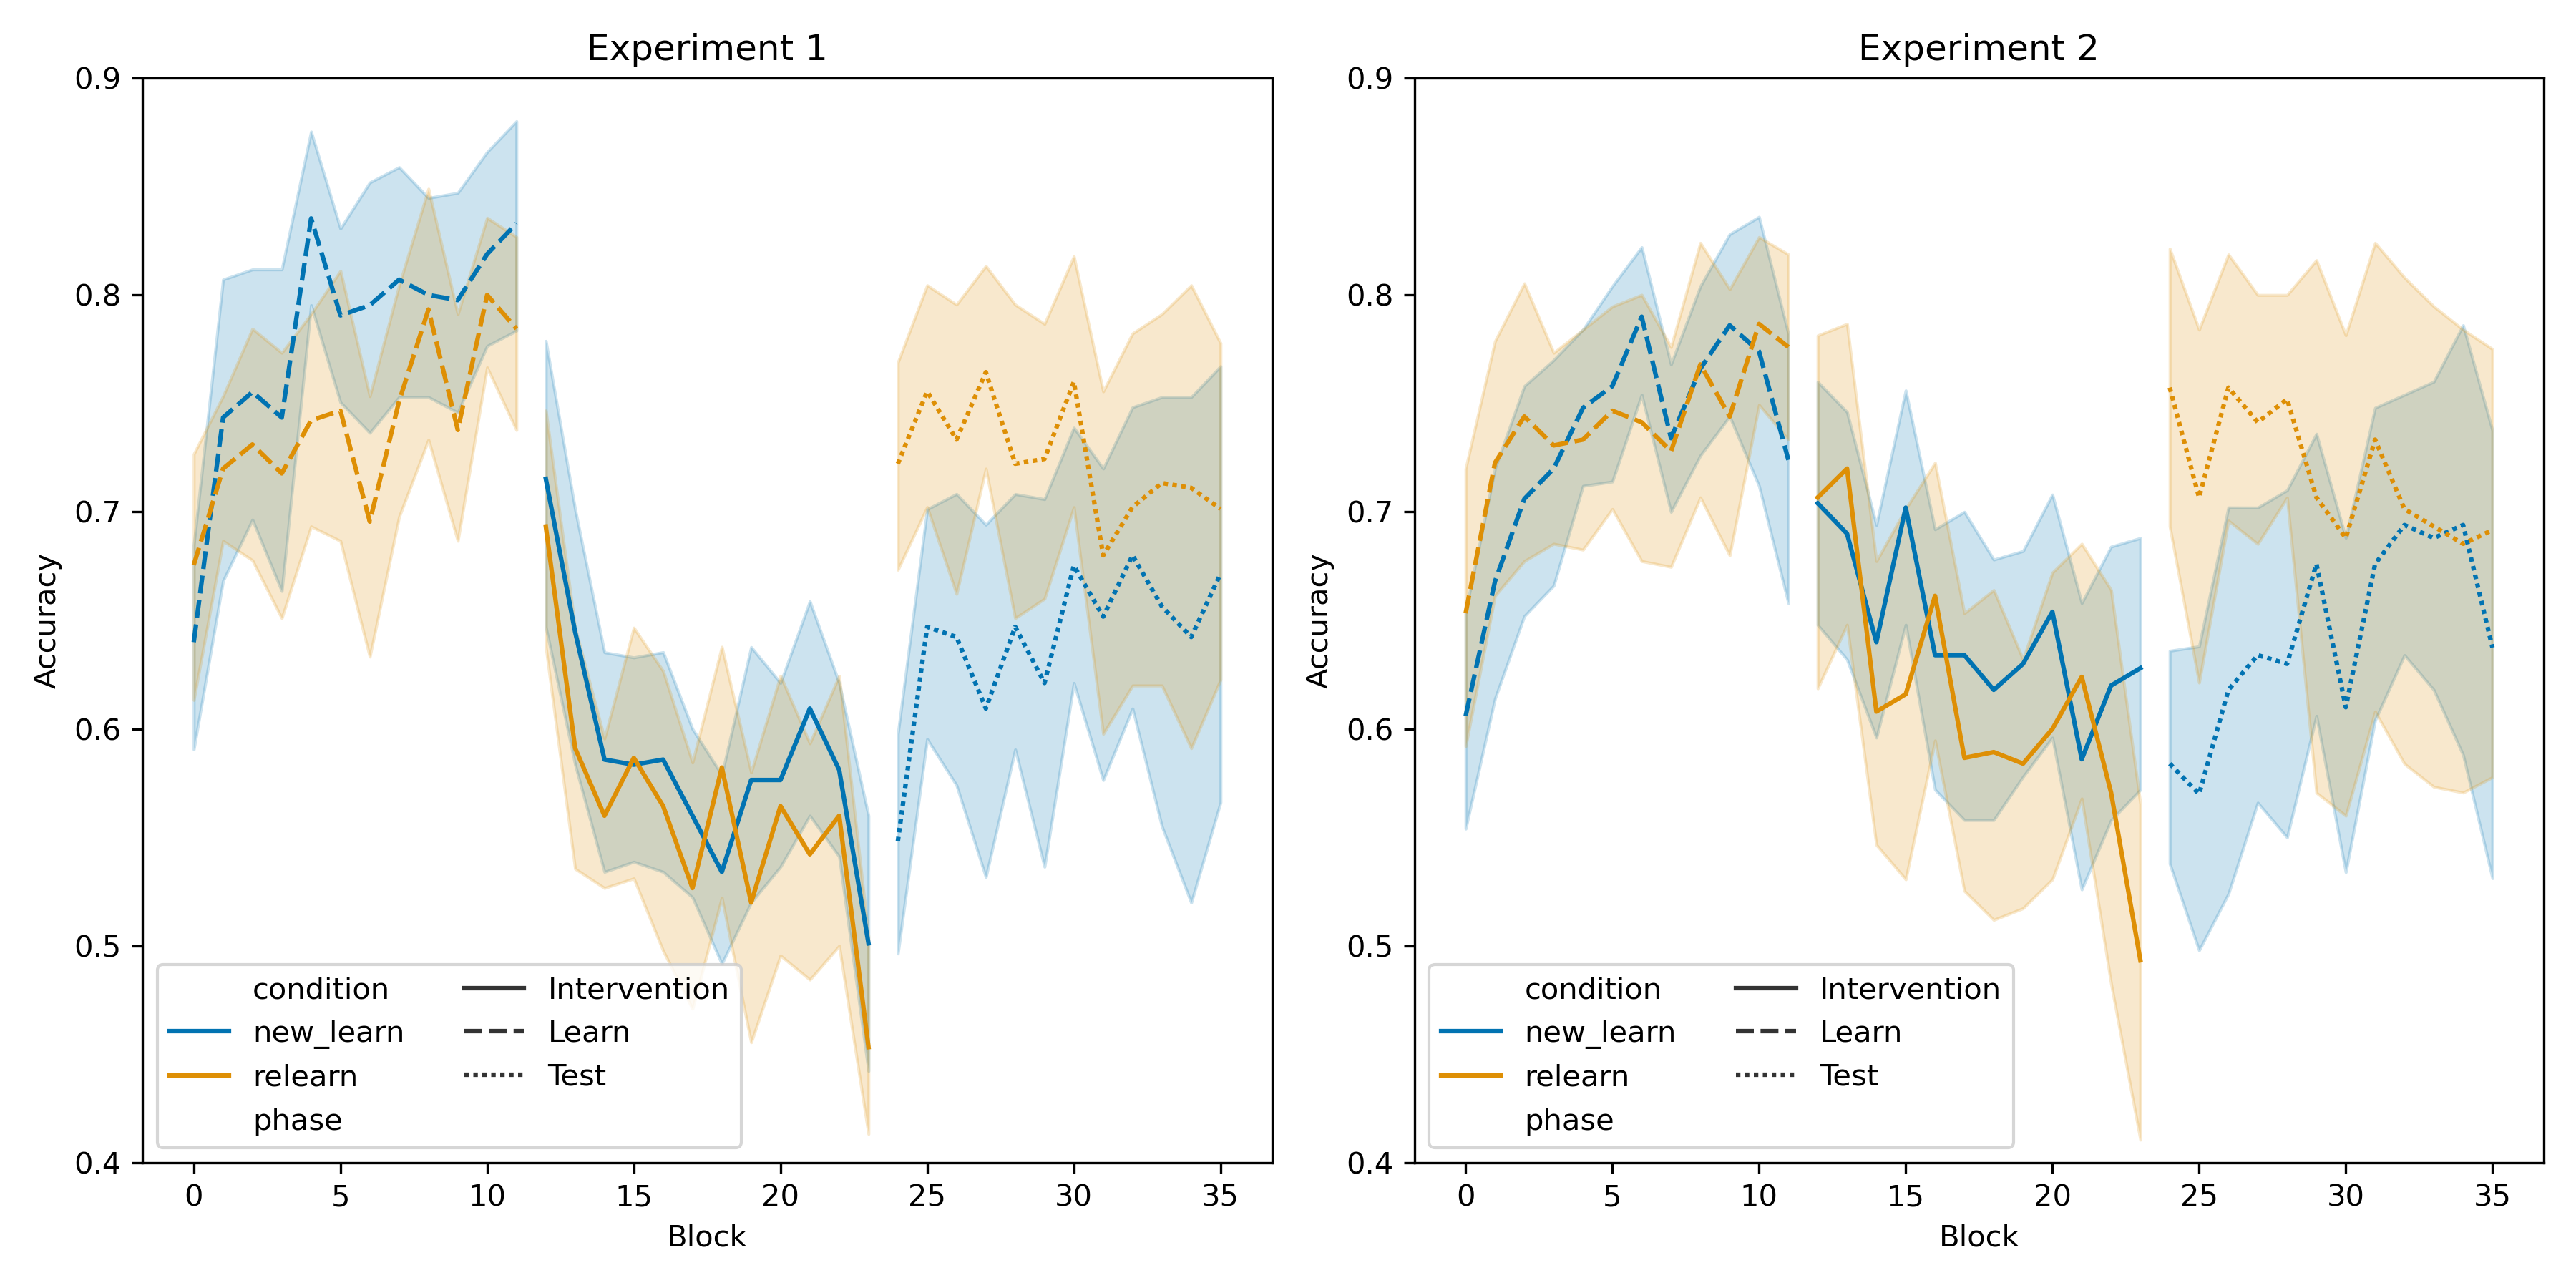
\includegraphics[width=\textwidth]{../figures/subjects_accuracy_all.png}
    \caption{
        Accuracy over blocks for all participants. Separate
        lines represent different conditions within each
        experiment.
}
\label{fig_learning_curves}
\end{figure}

Although the results suggest that the mixed-feedback
intervention leads to memory masking rather than
overwriting, it is essential to rule out potential
contamination by the declarative system (e.g., the use of
explicit rules). To address this, we fit decision-bound
models to each participant's data from the final block of
training and the first block of testing. Our primary
questions were: (1) did participants initially acquire a
procedural strategy, and (2) did they reacquire that
strategy during the Test phase? If the intervention caused
true unlearning, there should be no difference in the
proportion of participants expressing a procedural strategy
between the Relearn and New Learn conditions during the Test
phase.

Figure~\ref{fig_dbm_maps} shows heatmaps of transitions
between best-fit model classes from the end of training to
the start of testing, illustrating how participants shifted
(or failed to shift) their categorization strategies across
phases, separated by experiment and condition. In
Experiment~1, participants in the Relearn condition
predominantly acquired and reacquired a procedural strategy,
indicating that the intervention did not disrupt their
underlying category knowledge. In contrast, those in the New
Learn condition tended to switch from a procedural to a
rule-based strategy during the test phase, suggesting
interference rather than erasure. A similar pattern was
observed in Experiment~2. This further supports the
conclusion that an intervention of mixed feedback masks
rather than eliminates procedural category learning.

\begin{figure}[H]
    \centering
    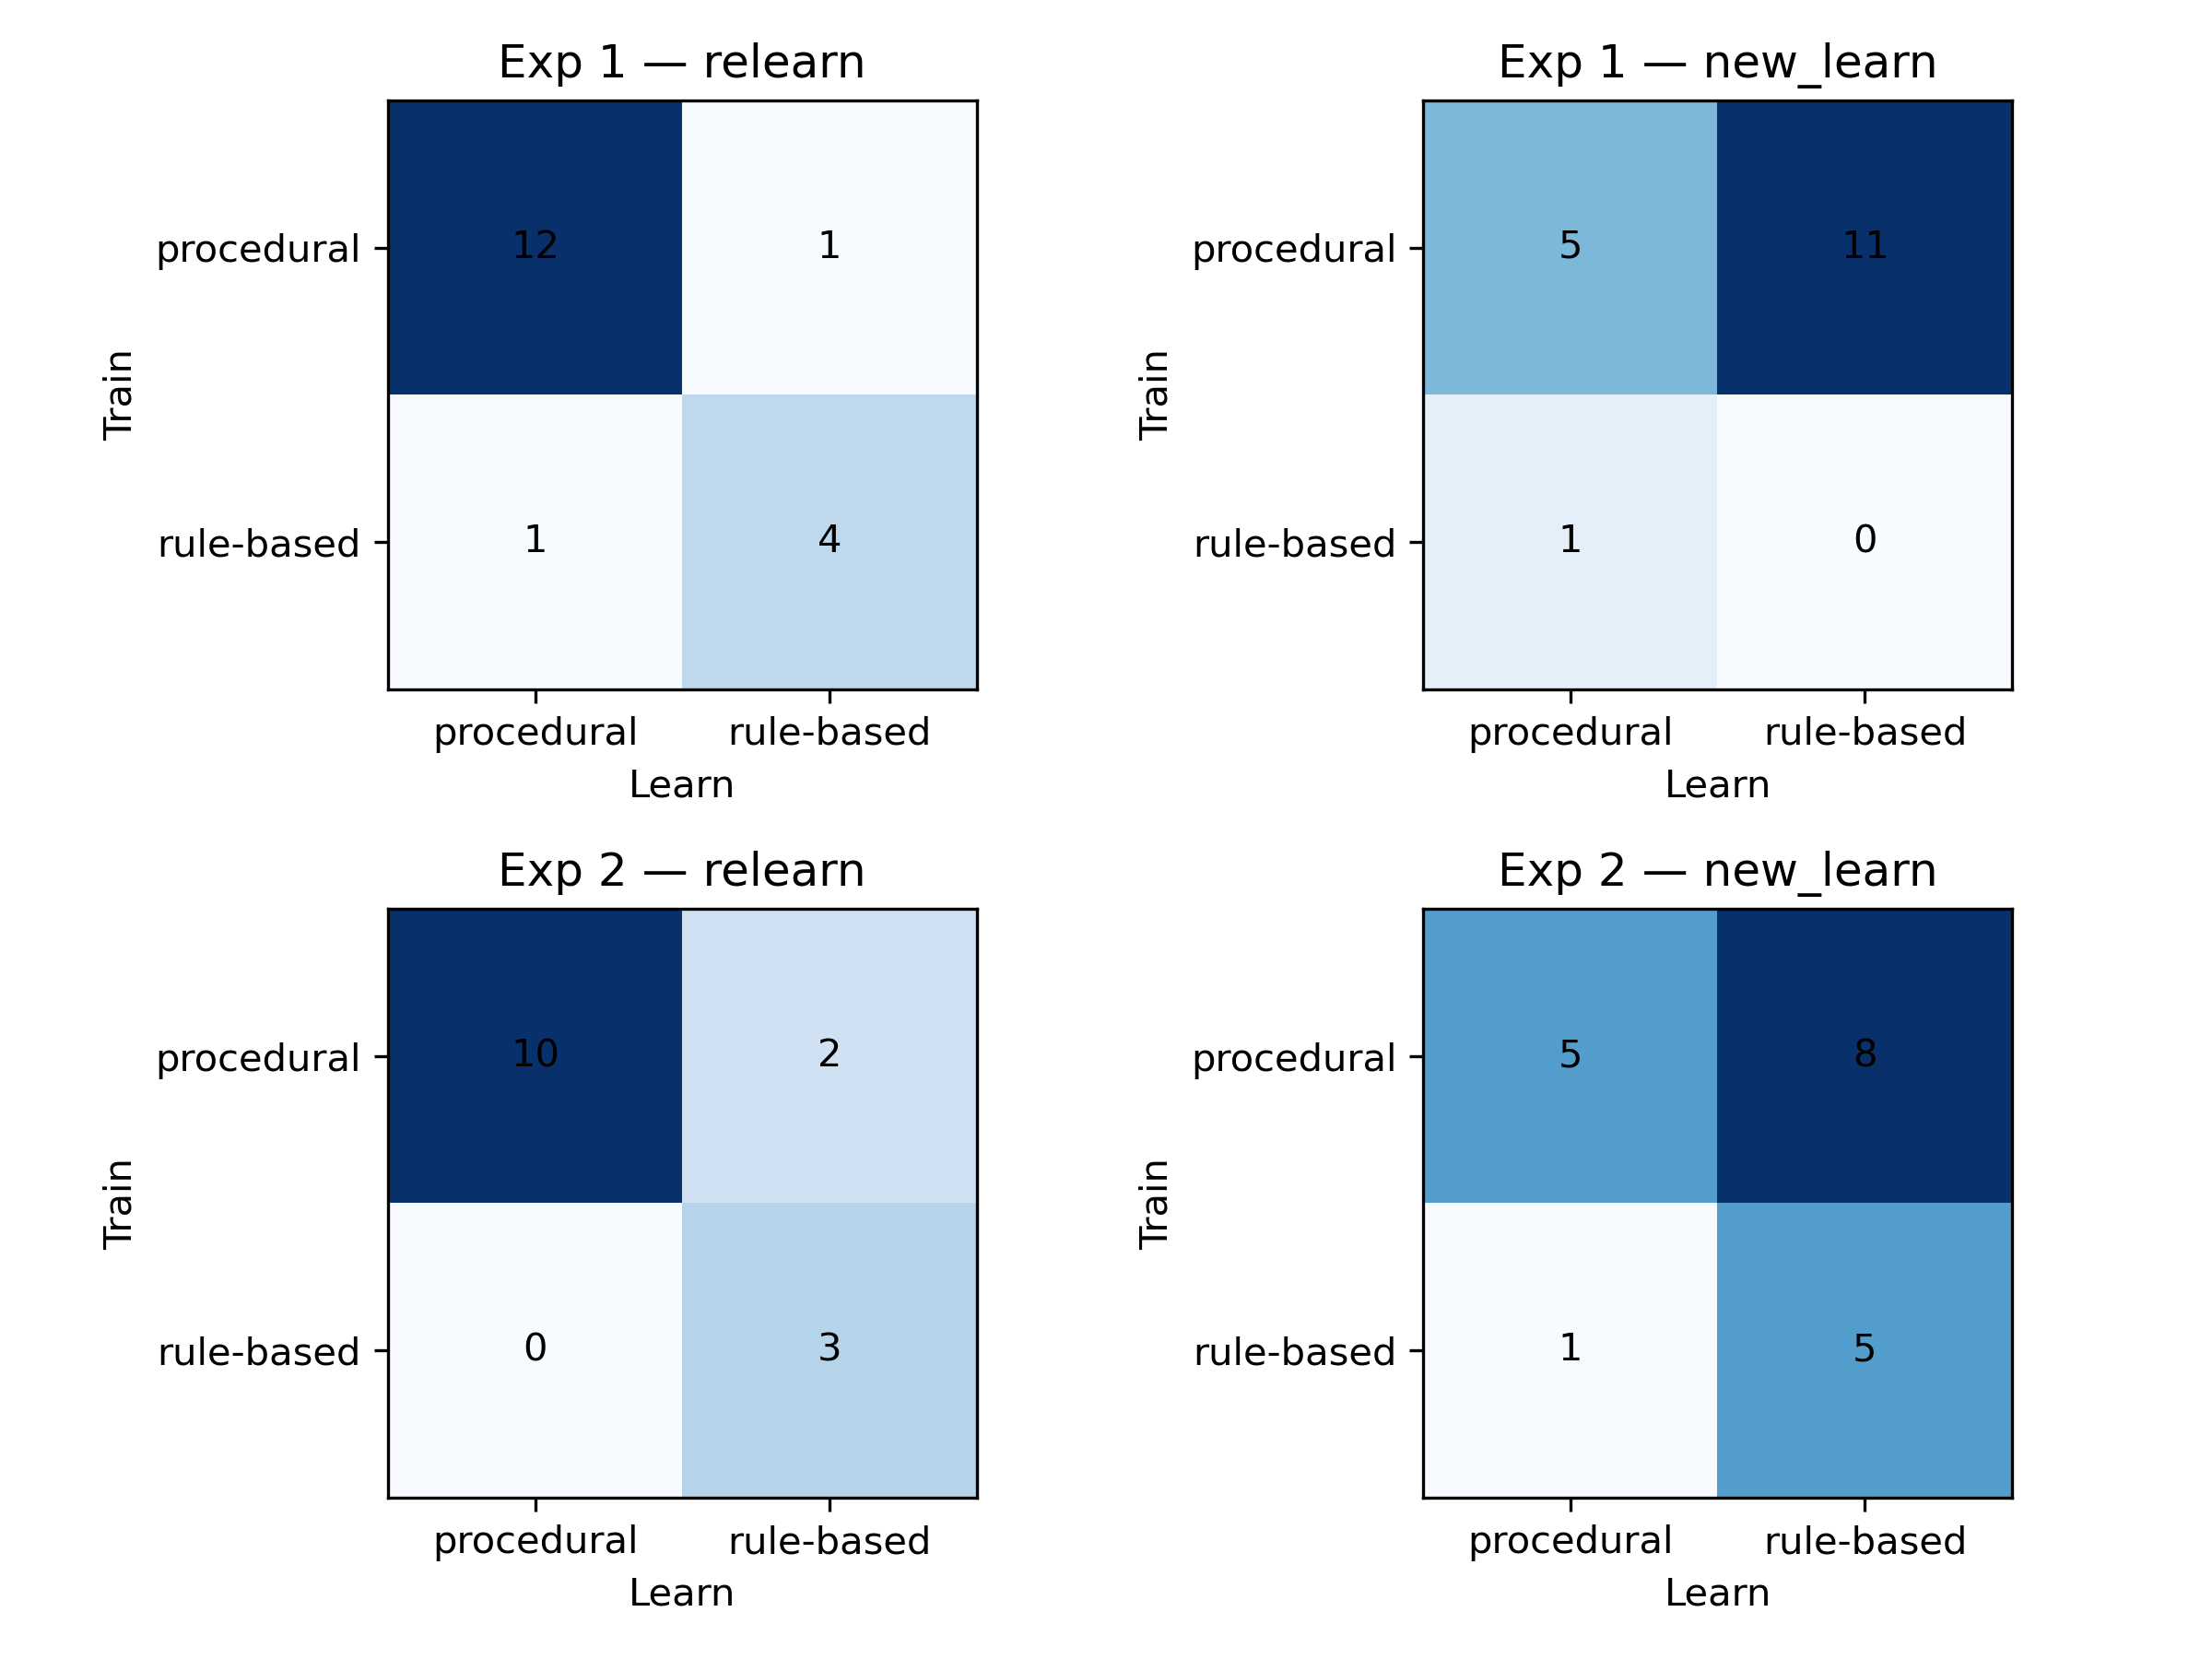
\includegraphics[width=\textwidth]{../figures/best_model_class_heatmap.png}
    \caption{
        Heatmaps showing transitions between best-fit model
        classes from the end of training (Y-axis) to the
        start of testing (X-axis), separated by experiment
        and condition. Each cell indicates the number of
        participants who transitioned between model classes.
}
\label{fig_dbm_maps}
\end{figure}

Figure~\ref{fig_dbm_stats} shows Bayesian posterior
estimates of the probability that participants reacquired a
procedural strategy during the initial stages of the Test
phase. For both the Relearn and New Learn conditions, there
was little difference in reacquisition probability between
Experiment~1 and Experiment~2, as indicated by the 95\%
credible intervals that included zero (top and middle rows,
rightmost panels). However, participants in the Relearn
condition were substantially more likely to reacquire a
procedural strategy than those in the New Learn condition.
This was true in both experiments, as shown by the 95\%
credible intervals excluding zero in the bottom row's left
and middle panels. Together, these results provide strong
evidence that the intervention masked but did not erase
procedural category knowledge.

\begin{figure}[H]
    \centering
    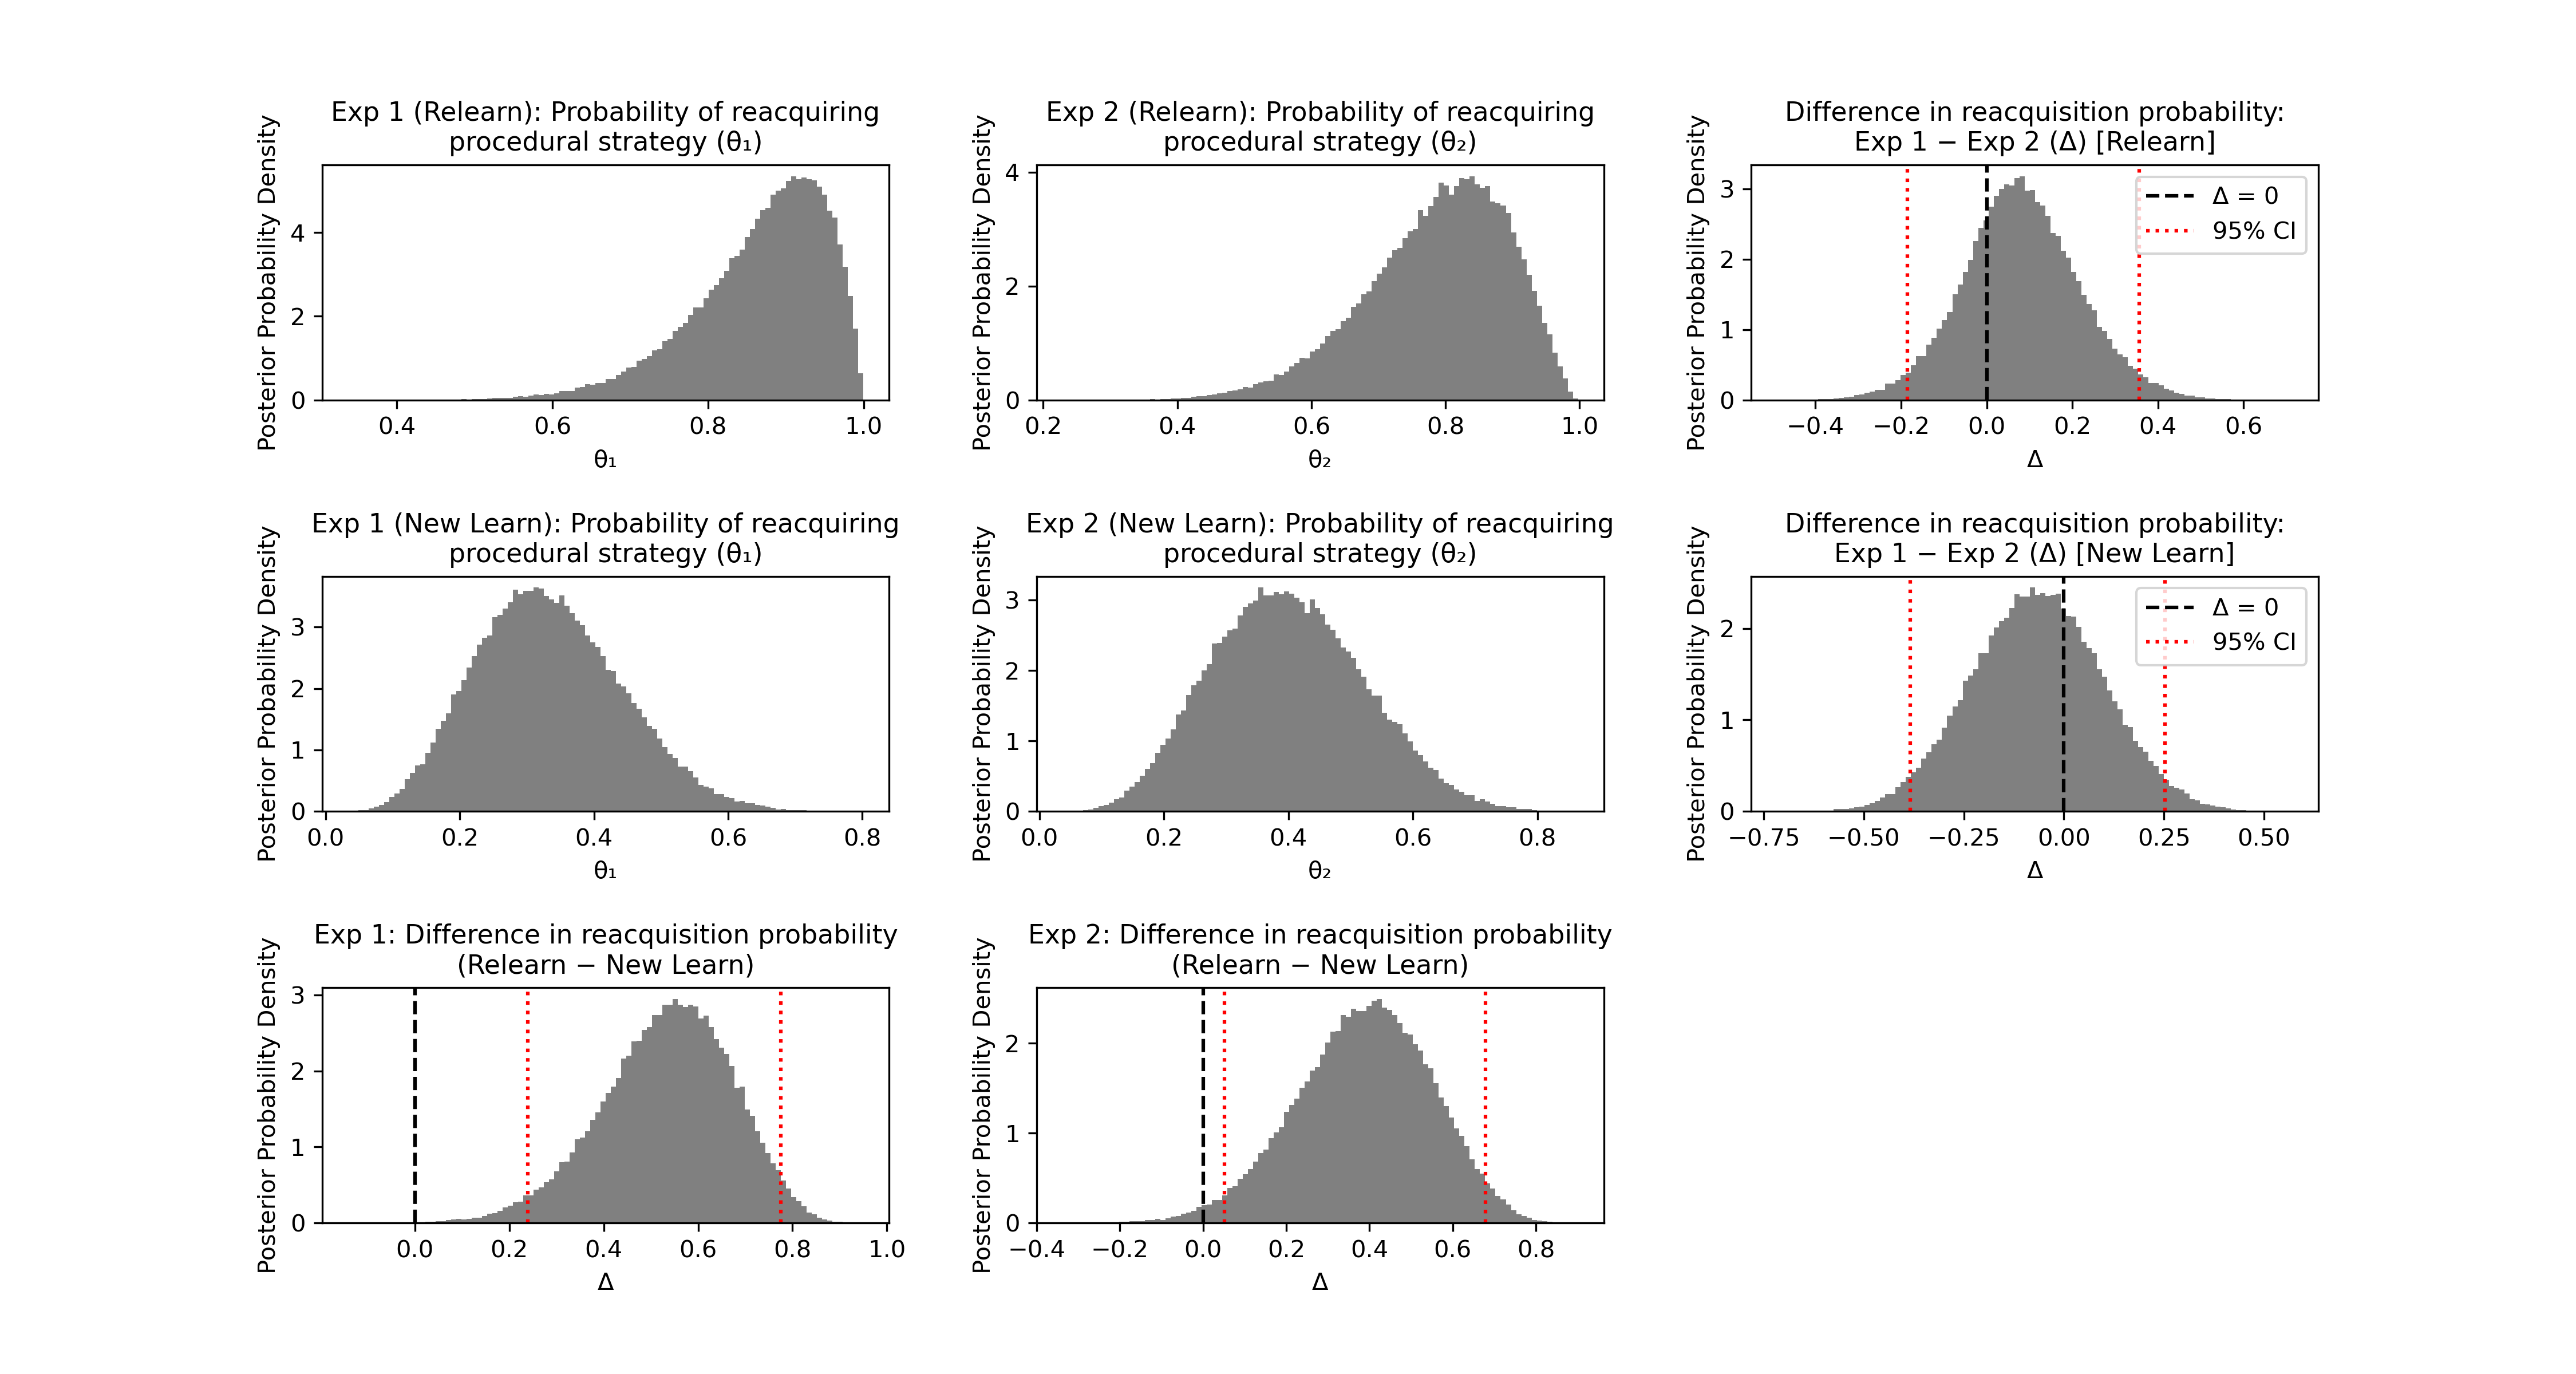
\includegraphics[width=\textwidth]{../figures/bayesian_comparison.png}
    \caption{
        Bayesian posterior distributions over $\theta$, the
        probability of reacquiring a procedural strategy.
        Top two rows show experiment comparisons within
        Relearn and New Learn conditions. Bottom row shows
        differences between conditions within each
        experiment. Red lines denote 95\% credible
        intervals; black dashed lines indicate null
        difference ($\Delta = 0$).
}
\label{fig_dbm_stats}
\end{figure}

\section{Discussion}
...

\end{document}

